\documentclass{scrartcl}
\usepackage[utf8]{inputenc}
\usepackage[spanish,es-tabla]{babel}	% Paquete de idiomas 'babel':
						%
						% 	Idioma: 'spanish'
						%	Opciones:
						%		es-tabla: sustituye la palabra 'cuadro' por 'tabla'.

\usepackage{amsmath,amsfonts,amsthm}
\usepackage{txfonts}	% Fuente Times
\renewcommand{\sectfont}{\rmfamily \bfseries} %cabeceras y titulos con estilo roman, negrita.


\usepackage{booktabs}	% Permite construir tablas de alta calidad.
\usepackage{tabu}
\usepackage{caption}
\usepackage{subcaption}
\usepackage{hyperref}
\usepackage{txfonts}
\usepackage{notoccite}
\usepackage{xspace}

\usepackage[thinspace,mediumqspace,squaren]{SIunits}	% Sistema Internacional de unidades.
	\newcommand{\micras}{\micro\meter\xspace}
	\newcommand{\mm}{\milli\meter\xspace}
	\newcommand{\cm}{\centi\meter\xspace}
	\newcommand{\nm}{\nano\meter\xspace}

	\newcommand{\Exp}[1]{\cdot\power{10}{#1}}
	\newcommand{\vect}[1]{\mathbf{#1}}

%% TikZ %%
%
\usepackage{tikz}
\usepackage{pgfplots}
\pgfplotsset{compat=1.3}


\usepackage{float}
\newfloat{grafica}{htbp}{log}
\floatname{grafica}{Gráfica}


%% TikZ %%
%
\usepackage{tikz}


\renewcommand{\thesubsection}{\thesection.\alph{subsection}}
\usepackage[makeroom]{cancel}

\title{Simulación del modelo de Ising en 2D}
\author{Ignacio Suárez Andrés}
\date{15 de junio de 2015}

\begin{document}
\maketitle
\section{Introducción}
Este ejercicio consiste en la implementación de una simulación del modelo de Ising en 2D para una red cuadrada. El sistema está descrito por el hamiltoniano
\begin{equation}
H=-J\sum_{<i,j>} s_i s_j
\end{equation}
donde $s_i$ y $s_j$ representan los spines de los puntos de la red y pueden tomar el valor +1 o -1. Tomamos el valor $J=1$ por simplicidad.\par
Se estudia el comportamiento a diferentes temperaturas, con unidades de $k_B=1$, es decir, $k_BT\equiv T$. La evolución del sistema se simula mediante el algoritmo de Metropolis, para una red cuadrada de 100$\times$100 puntos y 20000 pasos de tiempo, entendiendo un paso como un número de ciclos del algoritmo igual al número de puntos de la red.\par
El código, en C++ para la simulación y en R para la visualización, se encuentra disponible en \href{https://github.com/nachosandres/Ising2D}{GitHub}.

\section{Determinación de $T_c$}
Para conocer qué valores de $T$ tiene sentido analizar, conviene determinar primero la temperatura crítica. Con este fin, partimos de dos valores, $T=1$ y $T=3$ que comprobamos fácilmente que corresponden a los comportamientos ferromagnético y paramagnético respectivamente.\par
Recorremos los valores intermedios en intervalos de $\Delta T = 0.005$, realizando para cada uno la simulación con 20000 pasos de tiempo y extrayendo de cada una el promedio y la desviación estándar de la magnetización media del sistema, tomando para dicho promedio los últimos 10000 pasos. Se muestran los resultados en la figura \ref{fig:allT}, de donde se pueden extraer las siguientes conclusiones:\par
\begin{itemize}
\item Existe una temperatura crítica $T_c \approx$ 2,3 por debajo de la cual se da el comportamiento ferromagnético, con todos los spines tendiendo a orientarse en el mismo sentido, y por encima de la cual el comportamiento es paramagnético, con magnetización promedio aproximadamente nula.
\item La forma de la gráfica se corresponde con una bifurcación horquilla (o \textit{pitchfork}) supercrítica.
\item De las simulaciones con magnetización media mayor que 0,95 en valor absoluto, el 47\% (150) tienen valor positivo y el 53\% (168) negativo, valores cercanos al 50\% esperado. Se dan también, con $T<T_c$, estados en los que se forman dominios magnéticos y no llegan a tender a uno de los dos extremos, aunque sus fluctuaciones muestran que no son estables.
\item Las temperaturas altas dificultan la formación de pequeños dominios, reduciendo así cada vez más la probabilidad de alejarse del valor 0 mediante fluctuaciones.
\end{itemize}

\begin{figure}
\centering
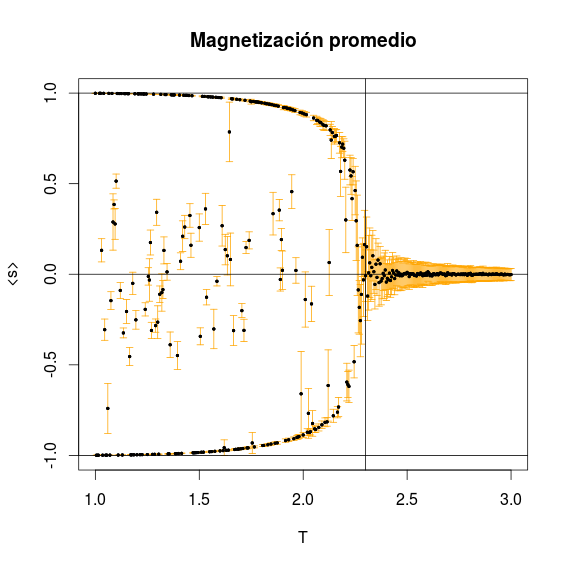
\includegraphics[scale=0.7]{allT}
\caption{Valores promedio de la magnetización para 400 valores de T, junto a la desviación estándar para representar las fluctuaciones dentro del periodo de tiempo recogido.}
\label{fig:allT}
\end{figure}




\clearpage
\section{Evolución temporal}
Para entender el efecto de la temperatura, es conveniente analizar la evolución de la magnetización media desde su inicialización aleatoria.\par
En la figura \ref{fig:tempnoTc} se han representado varios casos con temperaturas alejadas del punto crítico. Para $T<T_c$, la estabilización en torno a +1 o -1 es rápida, salvo para las excepciones en las que se forman dominios en el material. Para $T>T_c$, la magnetización media oscila cerca de 0. Se puede apreciar en ambos casos cómo la temperatura favorece el desorden, oponiéndose a la estabilización lejos de 0.\par
Por otra parte, en la figura \ref{fig:tempTc} se ha estudiado el comportamiento con temperaturas cercanas a $T_c$. Vemos cómo, partiendo de $T<T_c$ y subiendo, la magnetización media va dejando de estabilizarse en un valor extremo y va tomando valores menores, llegando hasta el punto de que para $T>T_c$ las oscilaciones se producen en torno a 0. Sin embargo, en torno a $T_c$, especialmente para $T=$ 2,3, las fluctuaciones se vuelven muy bruscas, pasando de golpe de estados con orientación mayoritariamente positiva a negativa y viceversa, sin alcanzar un punto de estabilidad en torno al cual oscilar.
\begin{figure}[ht]
\centering
\begin{subfigure}{.5\textwidth}
  \centering
  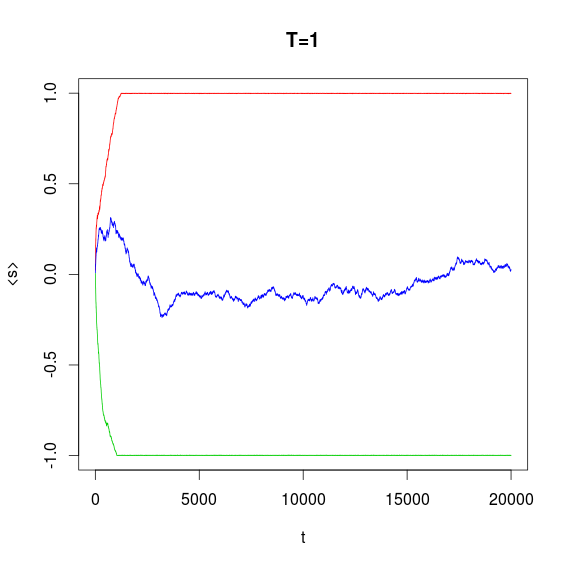
\includegraphics[width=1\linewidth]{T1}
\end{subfigure}%
\begin{subfigure}{.5\textwidth}
  \centering
  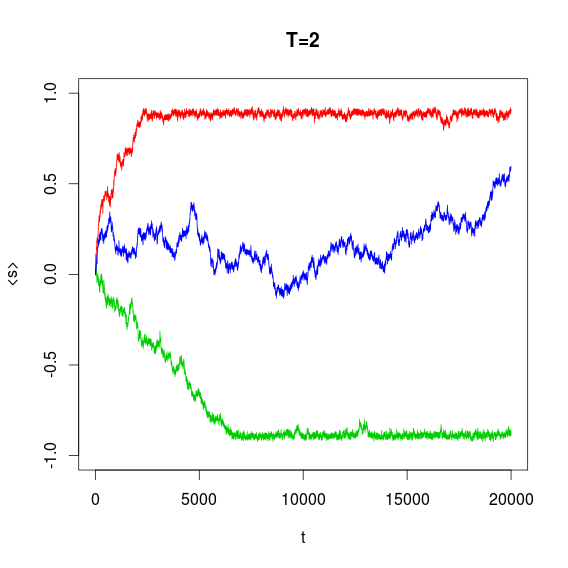
\includegraphics[width=1\linewidth]{T2}
\end{subfigure}
\begin{subfigure}{.5\textwidth}
  \centering
  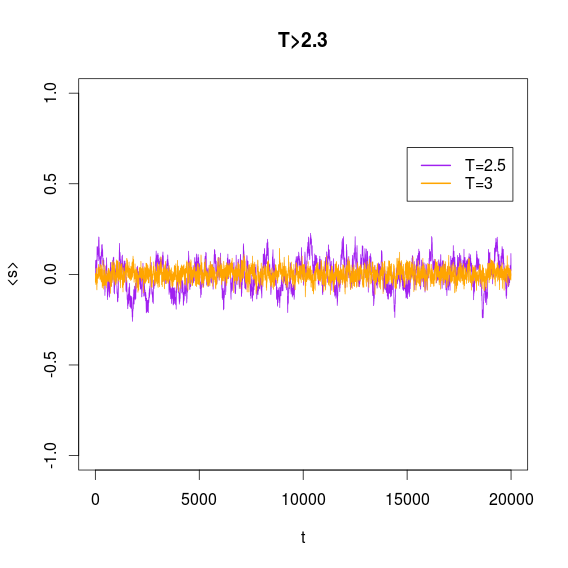
\includegraphics[width=1\linewidth]{T3}
\end{subfigure}
\caption{Evolución temporal de la magnetización media para diferentes temperaturas alejadas de $T_c$, representando en cada caso todos los comportamientos que pueden darse.}
\label{fig:tempnoTc}
\end{figure}

\begin{figure}[ht]
\centering
\begin{subfigure}{.6\textwidth}
  \centering
  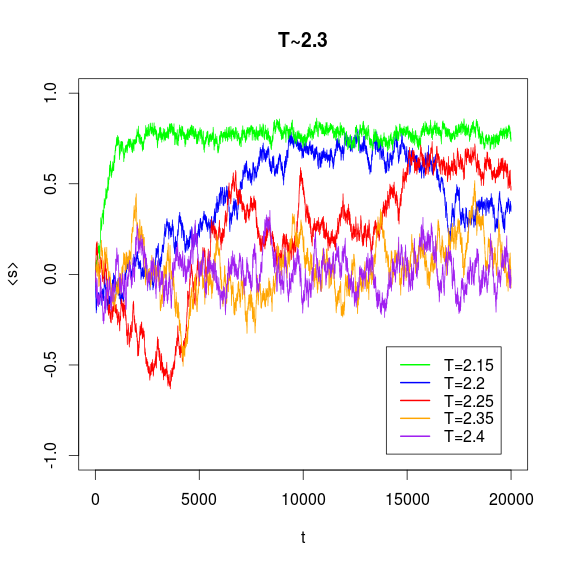
\includegraphics[width=1\linewidth]{Tno23}
\end{subfigure}
\begin{subfigure}{.6\textwidth}
  \centering
  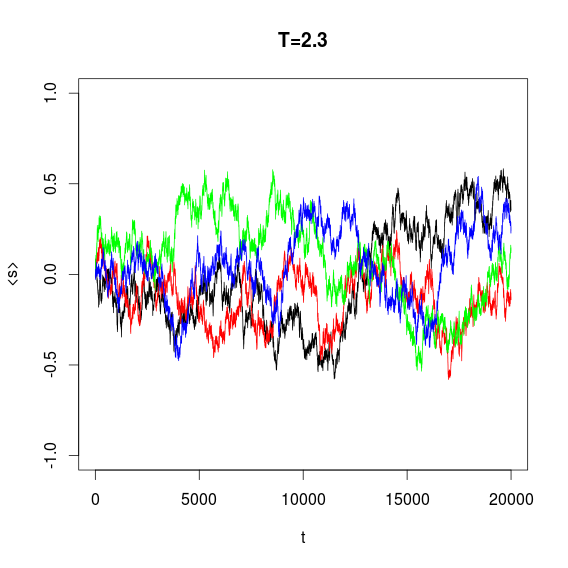
\includegraphics[width=1\linewidth]{T23}
\end{subfigure}
\caption{Evolución temporal de la magnetización media para temperaturas en torno a $T_c$, con especial detalle para $T=$ 2,3.}
\label{fig:tempTc}
\end{figure}

\clearpage
\section{Representación de la magnetización}
La distribución de spines del material simulado se puede comprender mediante una representación gráfica. Para ello, se han tomado los estados finales de las simulaciones mostradas en el apartado anterior.\par
En la figura \ref{fig:spinsmenorTc} se aprecia cómo, salvo formación de dominios que sean estables por sí mismos, se tiende a que una gran mayoría de los spines se orienten en el mismo sentido si $T<T_c$. Al aumentar la temperatura, aparecen cada vez más puntos que se oponen a la orientación mayoritaria, con un comportamiento cada vez más irregular al aproximarse a la temperatura crítica.\par
Para $T>T_c$, vemos en la figura \ref{fig:spinsmayorTc} cómo progresivamente van desapareciendo las regiones con spines acoplados entre sí, tendiendo al aumentar la temperatura a una distribución aleatoria.\par
Con $T=$ 2,3, el valor que hemos determinado como $T_c$, encontramos en la figura \ref{fig:spinsTc} un comportamiento que no encaja con lo visto generalmente en los casos anteriores. Concretamente, se observa que el material se llena de dominios cuyas fronteras siguen patrones irregulares
\begin{figure}[ht]
\centering
\begin{subfigure}{.35\textwidth}
  \centering
  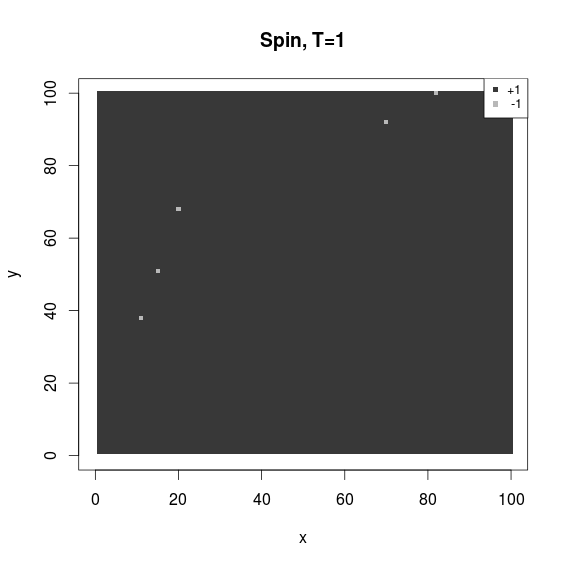
\includegraphics[width=1\linewidth]{spins/spinT1+}
\end{subfigure}%
\begin{subfigure}{.35\textwidth}
  \centering
  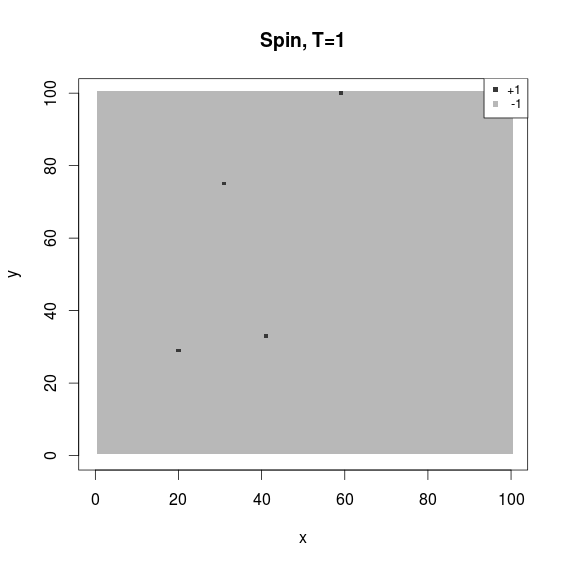
\includegraphics[width=1\linewidth]{spins/spinT1-}
\end{subfigure}%
\begin{subfigure}{.35\textwidth}
  \centering
  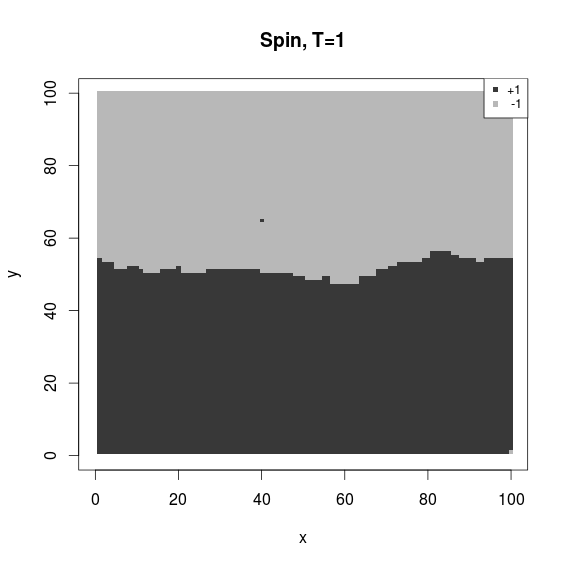
\includegraphics[width=1\linewidth]{spins/spinT1doms}
\end{subfigure}
\begin{subfigure}{.35\textwidth}
  \centering
  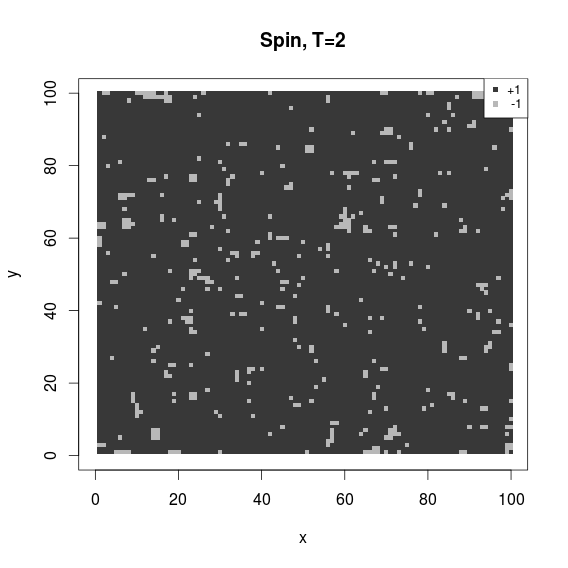
\includegraphics[width=1\linewidth]{spins/spinT2+}
\end{subfigure}%
\begin{subfigure}{.35\textwidth}
  \centering
  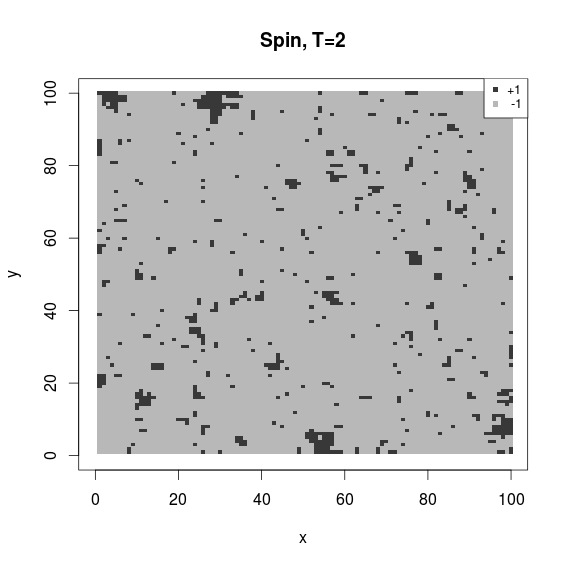
\includegraphics[width=1\linewidth]{spins/spinT2-}
\end{subfigure}%
\begin{subfigure}{.35\textwidth}
  \centering
  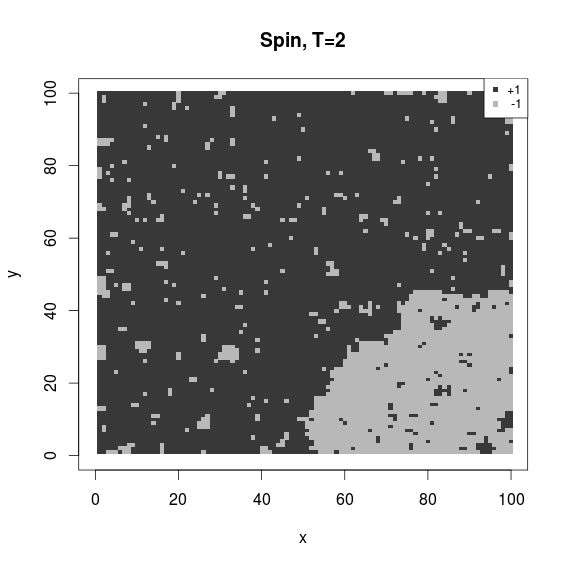
\includegraphics[width=1\linewidth]{spins/spinT2doms}
\end{subfigure}
\begin{subfigure}{.35\textwidth}
  \centering
  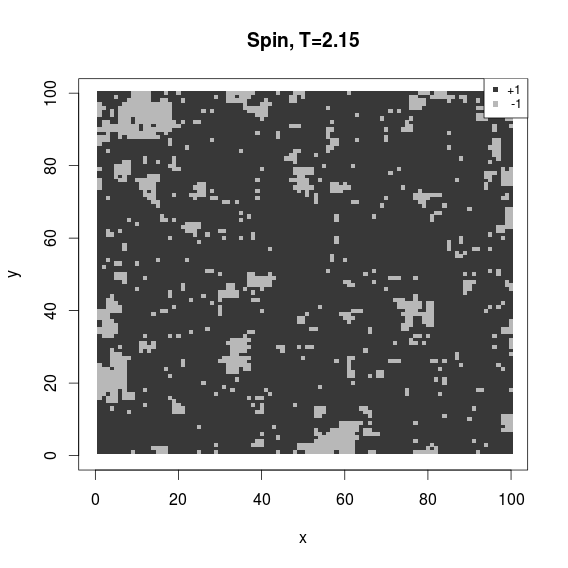
\includegraphics[width=1\linewidth]{spins/spinT2_15}
\end{subfigure}%
\begin{subfigure}{.35\textwidth}
  \centering
  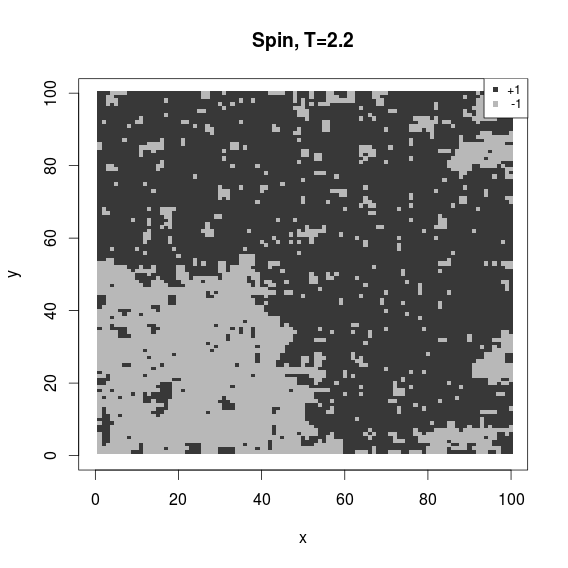
\includegraphics[width=1\linewidth]{spins/spinT2_2}
\end{subfigure}%
\begin{subfigure}{.35\textwidth}
  \centering
  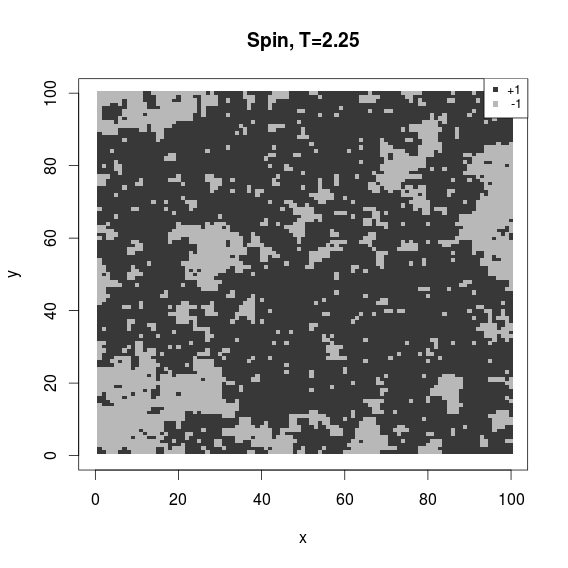
\includegraphics[width=1\linewidth]{spins/spinT2_25}
\end{subfigure}
\caption{Estado final de la magnetización para temperaturas inferiores a $T_c$. Para los valores 1 y 2, se muestran los estados de orientación positiva y negativa, junto a un ejemplo de formación de dominios estables.}
\label{fig:spinsmenorTc}
\end{figure}

\begin{figure}[ht]
\centering
\begin{subfigure}{.35\textwidth}
  \centering
  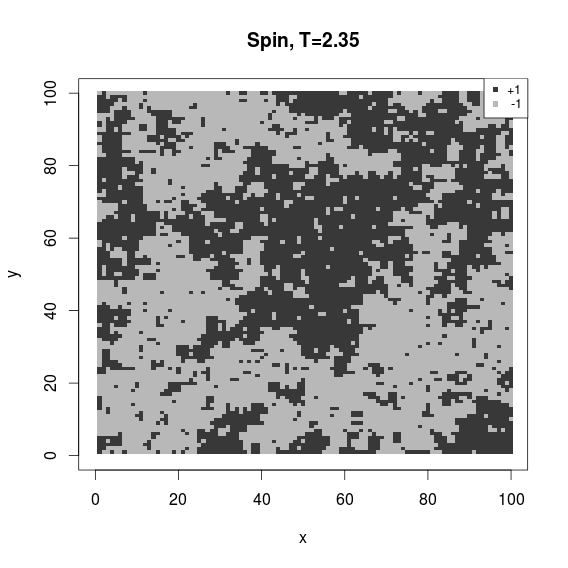
\includegraphics[width=1\linewidth]{spins/spinT2_35}
\end{subfigure}%
\begin{subfigure}{.35\textwidth}
  \centering
  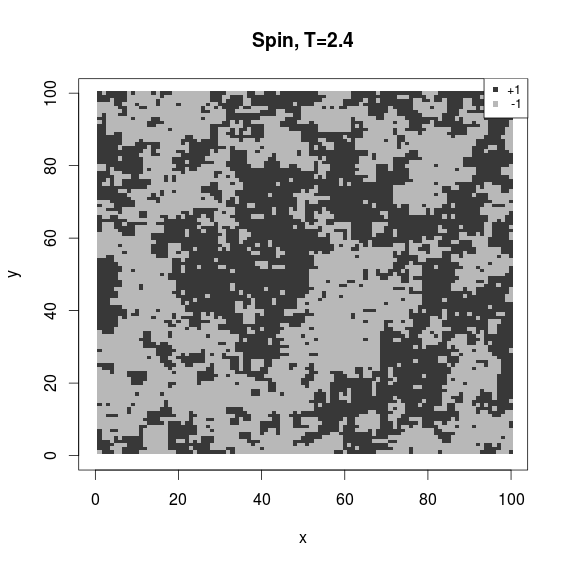
\includegraphics[width=1\linewidth]{spins/spinT2_4}
\end{subfigure}%
\begin{subfigure}{.35\textwidth}
  \centering
  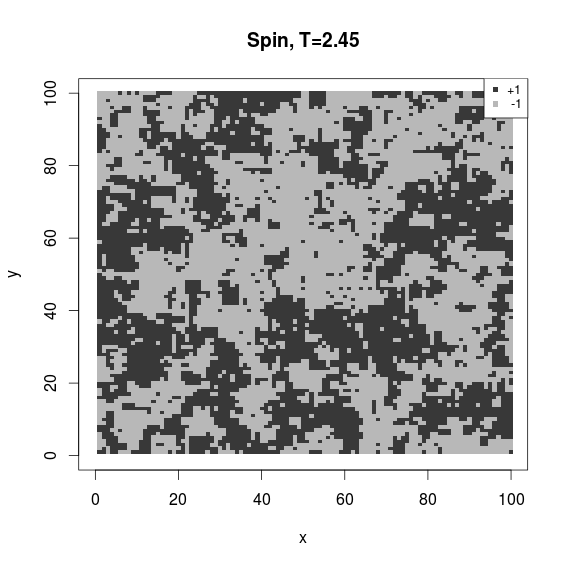
\includegraphics[width=1\linewidth]{spins/spinT2_45}
\end{subfigure}
\begin{subfigure}{.35\textwidth}
  \centering
  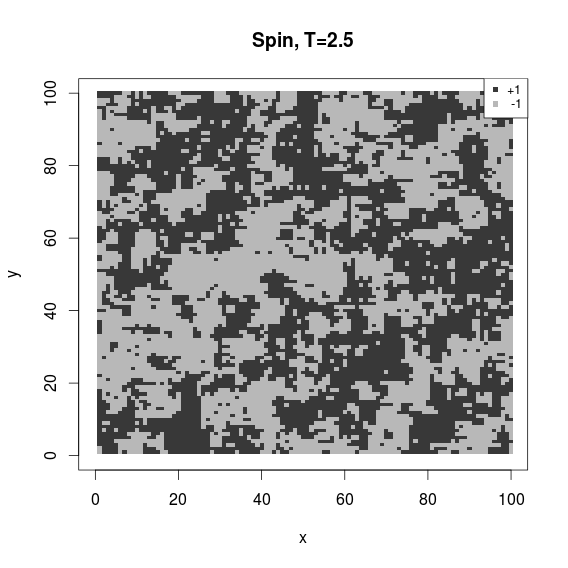
\includegraphics[width=1\linewidth]{spins/spinT2_5}
\end{subfigure}%
\begin{subfigure}{.35\textwidth}
  \centering
  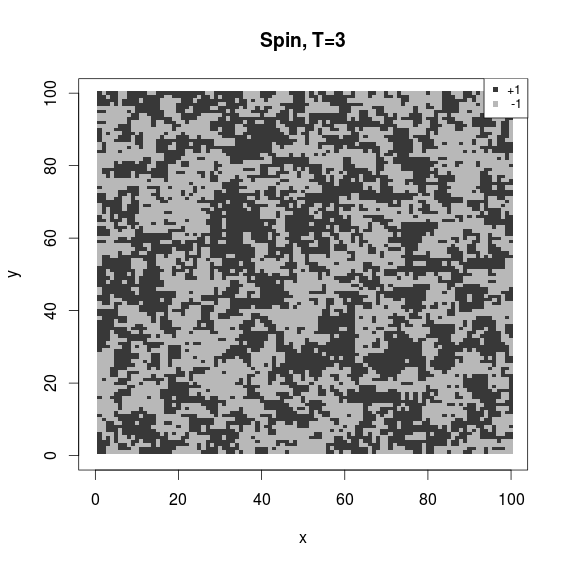
\includegraphics[width=1\linewidth]{spins/spinT3}
\end{subfigure}
\caption{Estado final de la magnetización para varias temperaturas superiores a $T_c$.}
\label{fig:spinsmayorTc}
\end{figure}

\begin{figure}[ht]
\centering
\begin{subfigure}{.5\textwidth}
  \centering
  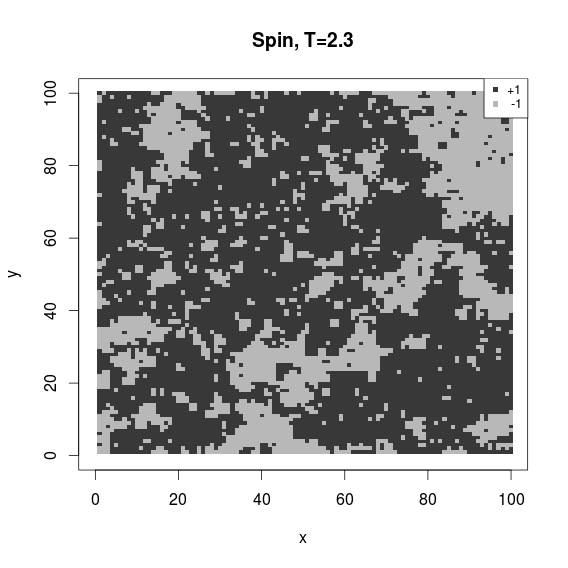
\includegraphics[width=1\linewidth]{spins/spinT2_3_1}
\end{subfigure}%
\begin{subfigure}{.5\textwidth}
  \centering
  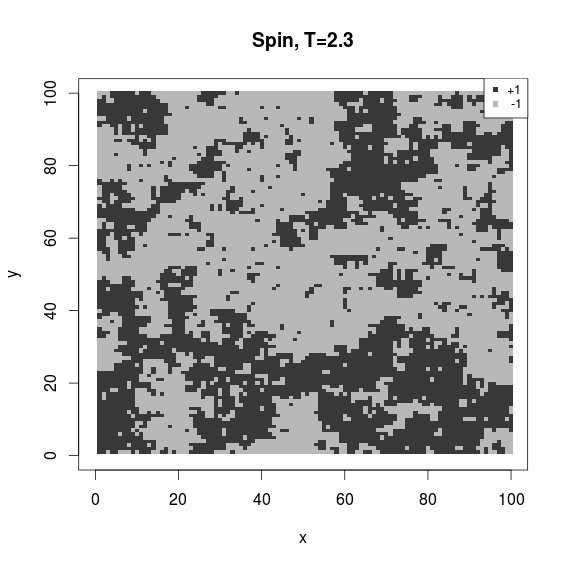
\includegraphics[width=1\linewidth]{spins/spinT2_3_2}
\end{subfigure}
\begin{subfigure}{.5\textwidth}
  \centering
  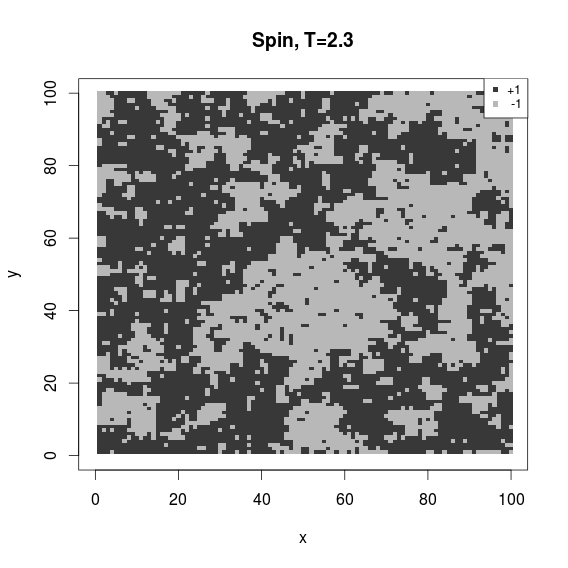
\includegraphics[width=1\linewidth]{spins/spinT2_3_3}
\end{subfigure}%
\begin{subfigure}{.5\textwidth}
  \centering
  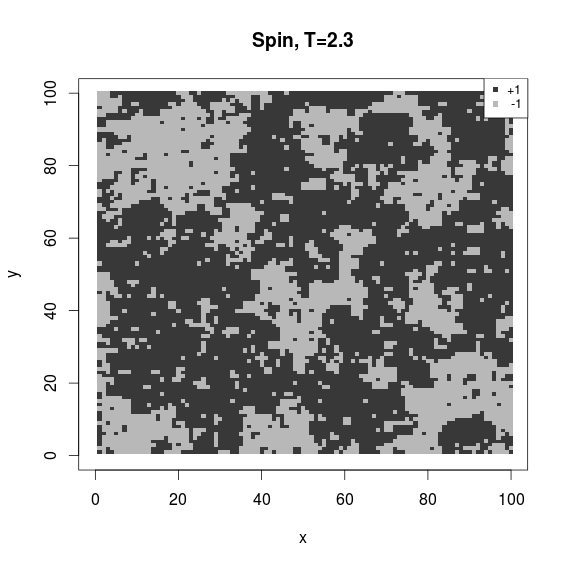
\includegraphics[width=1\linewidth]{spins/spinT2_3_4}
\end{subfigure}
\caption{Estado final de la magnetización para $T=T_c=$ 2,3. Se muestran los resultados de cuatro simulaciones distintas, para descartar que no sea representativo.}
\label{fig:spinsTc}
\end{figure}

\clearpage
\section{Conclusiones}
\begin{itemize}
\item Se ha implementado una simulación del modelo de Ising en 2D para una red cuadrada de 100$\times$100 puntos con el algoritmo de Metropolis, con representaciones gráficas de los resultados.
\item Se ha encontrado aproximadamente la temperatura crítica del sistema, $T_c \approx$ 2,3, en unidades de $k_B=1$ y para $J=1$.
\item Por debajo de $T_c$ se ha observado que generalmente los spines tienden a orientarse todos en el mismo sentido en pocos pasos, con probabilidad de elección entre +1 o -1 del orden del 50\%.
\item Por encima de $T_c$, la temperatura desacopla los spines, dando lugar a una distribución aleatoria de promedio 0.
\item Para $T=T_c$, se forman patrones irregulares en las fronteras de los dominios, con fluctuaciones bruscas que cambian rápidamente el signo de la magnetización media y sin mostrar signos de poder tender a un estado estable.
\end{itemize}


\end{document}